\documentclass[tikz]{standalone}
% ------- TikZ Preamble -------
\RequirePackage{tikz}
\usetikzlibrary{knots, hobby,decorations.markings,calc,intersections, decorations.pathreplacing, shapes.geometric,spath3, decorations.pathreplacing}
% ------- Shared styles (from your preamble) -------
\tikzset{
    knot diagram/every strand/.append style={ultra thick, black},
}

% ------- Guides toggle -------
\newif\ifsstguides
\sstguidestrue

% ------- Helper: label & skeleton for points P1..Pn -------
\newcommand{\SSTGuidesPoints}[2]{% #1=basename (e.g. P), #2=last index
  \ifsstguides
    \foreach \i in {1,...,#2}{
      \fill[blue] (#1\i) circle (1.2pt);
      \node[blue,font=\scriptsize,above] at (#1\i) {\i};
    }
    \draw[gray!40, dashed]
    \foreach \i [remember=\i as \lasti (initially 1)] in {2,...,#2,1} { (#1\lasti)--(#1\i) };
  \fi
}

\begin{document}

    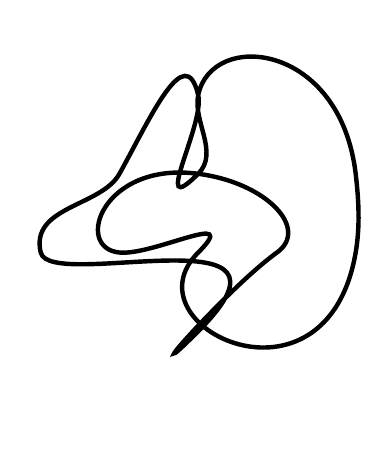
\begin{tikzpicture}[use Hobby shortcut]
    \coordinate (P1) at (0, 1);
    \coordinate (P2) at (-1, 1);
    \coordinate (P3) at (0, 2);
    \coordinate (P4) at (1, 1);
    \coordinate (P5) at (0, 0);
    \coordinate (P6) at (0, 0);
    \coordinate (P7) at (-2, 1);
    \coordinate (P8) at (-1, 2);
    \coordinate (P9) at (0, 3);
    \coordinate (P10) at (0, 2);
    \coordinate (P11) at (0, 2);
    \coordinate (P12) at (0, 3);
    \coordinate (P13) at (2, 2);
    \coordinate (P14) at (2, 1);
    \coordinate (P15) at (0, 1);
    \coordinate (P16) at (0, 1); % = P1

    \begin{knot}[
   consider self intersections,
    clip width=5pt,
    clip radius=3pt,
    ignore endpoint intersections=true,
        flip crossing/.list={2,4,6,8,10,12,14,16,18}    % draft mode=crossings % uncomment to see numbers
    ]
    \strand
    ([closed] P1)..(P2)..(P3)..(P4)..(P5)..(P6)..(P7)..(P8)..(P9)..(P10)..(P11)..(P12)..(P13)..(P14)..(P15)..(P16);
    \end{knot}
        \SSTGuidesPoints{P}{15}
\end{tikzpicture}
%
%\begin{tikzpicture}[use Hobby shortcut, line cap=round, line join=round, scale=1.05]
%
%% ---- controls ----
%\def\Amp{0.13}
%\def\Turns{4}        % can be non-integer; extrema logic still works
%\def\Samples{400}
%\def\Wth{2.5pt}
%\def\Core{black}     % set to page color for clean masking
%\def\Mask{5.0pt}
%\def\ClrA{black!60!black}
%\def\ClrB{red!70!black}
%
%\tikzset{
%  fat strand/.style={
%    draw=#1, line width=\Wth,
%    double=\Core, double distance=1.2*\Wth
%  }
%}
%
%% ---- coordinates ----
%\coordinate (P1) at (-2.0,-2.0);
%\coordinate (P2) at (-2.0, 2.0);
%\coordinate (P3) at ( 1.0,-0.5);
%\coordinate (P4) at (-1.0,-0.5);
%\coordinate (P5) at ( 2.0, 2.0);
%\coordinate (P6) at ( 2.0,-2.0);
%\coordinate (P7) at (-1.0, 0.5);
%\coordinate (P8) at ( 1.0, 0.5);
%\coordinate (P9) at (-2.0,-2.0); % = P1
%\def\KPATH{([closed] P1)..(P2)..(P3)..(P4)..(P5)..(P6)..(P7)..(P8)..(P9)}
%
%% ---- build two offset coordinate lists ----
%\newcommand{\MakeStrandCoords}[5]{%
%  \pgfmathtruncatemacro{\Ns}{#2}
%  \def\Phase{0}\ifx#5B\def\Phase{0.5}\fi
%  \foreach \i in {0,...,\Ns}{%
%    \pgfmathsetmacro{\s}{\i/\Ns}%
%    \pgfmathsetmacro{\y}{#3*sin(360*(#4*\s + \Phase))}%
%    \path[postaction={decorate, decoration={markings,
%      mark=at position \s with {\coordinate (#5\i) at (0,\y);}}}] #1;%
%  }%
%}
%\MakeStrandCoords{\KPATH}{\Samples}{\Amp}{\Turns}{A}
%\MakeStrandCoords{\KPATH}{\Samples}{\Amp}{\Turns}{B}
%
%% ---- segment drawer with overpass mask ----
%\newcommand{\drawSeg}[4]{% name(A/B), i, color, over(0/1)
%  \ifnum#4=1
%    \draw[preaction={draw=\Core, line width=\Mask}, fat strand=#3]
%      (#1#2) .. (#1\the\numexpr#2+1\relax);
%  \else
%    \draw[fat strand=#3]
%      (#1#2) .. (#1\the\numexpr#2+1\relax);
%  \fi
%}
%
%% ---- swap at offset extrema (least visible) ----
%\pgfmathtruncatemacro{\Last}{\Samples-1}
%\foreach \k in {0,...,\Last}{
%  \pgfmathsetmacro{\s}{\k/\Samples}
%  % block index changes at s = (1/4 + n/2)/Turns  <=> when 2*Turns*s crosses half-integers
%  \pgfmathtruncatemacro{\blk}{floor(2*\Turns*\s + 0.5)}
%  \ifodd\blk
%    % B over, A under
%    \drawSeg{A}{\k}{\ClrA}{0}
%    \drawSeg{B}{\k}{\ClrB}{1}
%  \else
%    % A over, B under
%    \drawSeg{B}{\k}{\ClrB}{0}
%    \drawSeg{A}{\k}{\ClrA}{1}
%  \fi
%}
%
%\end{tikzpicture}
\end{document}
